\documentclass[12pt,a4paper,openany]{memoir}
\usepackage[utf8]{inputenc}
\usepackage[german]{babel}
\usepackage[german]{isodate}
\usepackage{hyperref}
\usepackage{graphicx}
\usepackage{xcolor}
\usepackage{wrapfig}


\makeatletter
\def\thickhrulefill{\leavevmode \leaders \hrule height 1pt\hfill \kern \z@}
\renewcommand{\maketitle}{\begin{titlingpage}%
    \let\footnotesize\small
    \let\footnoterule\relax
    \parindent \z@
    \reset@font
    \null\vfil
    \begin{flushleft}
      \huge \@title
    \end{flushleft}
    \par
    \hrule height 4pt
    \par
    \begin{flushright}
      \LARGE \@author \par
    \end{flushright}
    \vskip 60\p@
    \vfil\null
  \end{titlingpage}%
  \setcounter{footnote}{0}%
}


\makeatother
\title{Raspberry Webradio Benutzerhandbuch}
\author{Michael Schwarz}

\begin{document}
\maketitle

\chapterstyle{ell}
\tableofcontents

\chapter{Einleitung}
Dies ist das offizielle Benutzerhandbuch zum Raspberry Webradio, einem selbstbau SHOUTcast streaming Radio auf Basis des Raspberry Pi.

Das Projekt ist auf \url{http://code.google.com/p/raspberry-webradio/} zu finden, wo auch der zugehörige Source Code und Schaltplan zur Verfügung stellt.

Das Raspberry Webradio dient dazu, SHOUTcast Radio Stationen ohne einen Computer wiedergeben zu können. Weiters ist es auch möglich, Musik von USB-Medien wiederzugeben. 

Die Verbindung zum Internet kann dabei sowohl über LAN als auch über WLAN erfolgen. 

Die Funktionalität wird im Kapitel \textit{Software} beschrieben. Das Gerät kann auch mit Hilfe eines Android Smartphones oder Tablets ferngesteuert werden. 
Mehr dazu ist im Kapitel \textit{Fernsteuerung} zu finden. 


\section{Kompatibilität}
Das Raspberry Webradio unterstützt SHOUTcast MP3 Streams und lokale MP3 Dateien, sowie M3U Playlists. 
Der Zugang zum Internet wird sowohl über LAN als auch über WLAN unterstützt. 

\chapter{Hardware}
 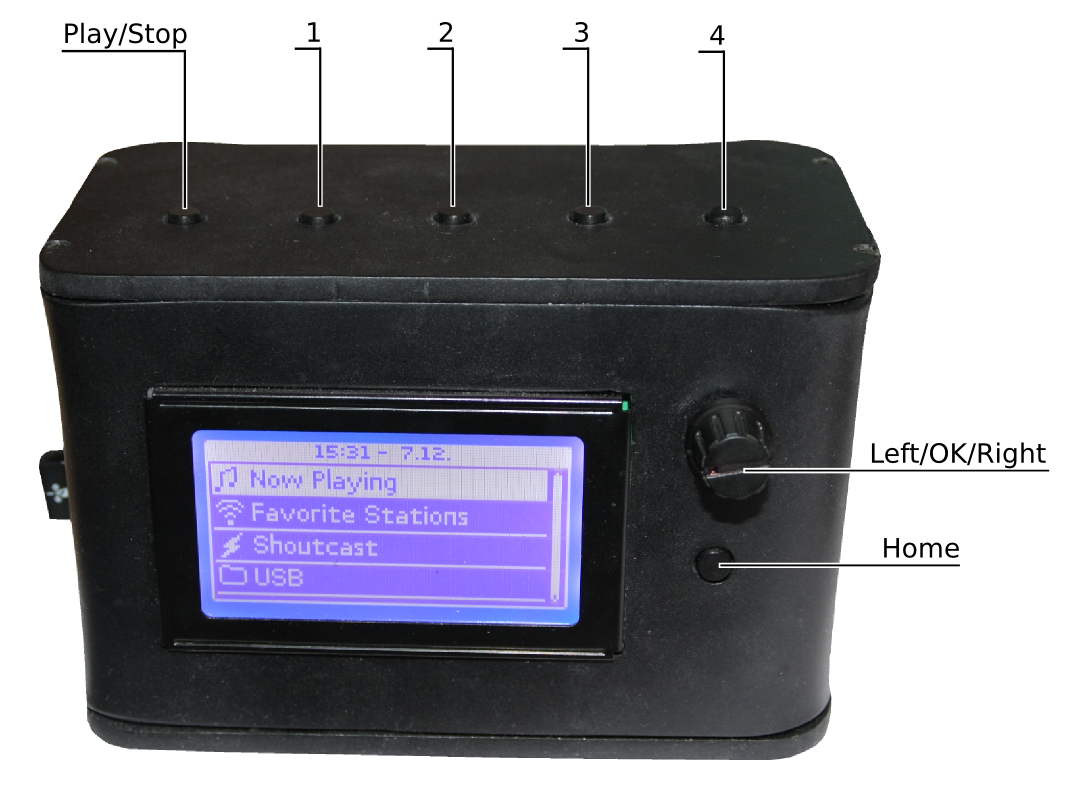
\includegraphics[width=120mm]{images/buttons.png}

\begin{itemize}
 \item \textbf{Home} kehrt von überall wieder ins Hauptmenü zurück.
 \item \textbf{Links/OK/Rechts}: Drehen des Knopfes wird zum Auswählen von Menüpunkten verwendet, ein Druck auf den Knopf bestätigt eine Auswahl.
 \item \textbf{Play/Stop}: Stoppt die Wiedergabe eines Streams. Im USB Modus wird der aktuell markierte Ordner abgespielt.
 \item \textbf{1/2/3/4}: Spielt den Stream der als Favorit Nummer 1/2/3/4 markiert ist. In der Stationsliste markiert langes Drücken der Taste den markierten Stream als Nummer 1/2/3/4.
\end{itemize}

\section{Stromversorgung}
Die Stromversorgung erfolgt über ein Netzteil mit 5 Volt und 1 Ampere. Der Stromverbrauch liegt bei durchschnittlich 3,5 Watt. 

\section{USB}
Der Raspberry Webradio stellt zwei USB Ports zur Verfügung. Davon kann einer für ein USB-Medium genutzt werden kann, von dem die Musikwiedergabe erfolgt. Es werden USB-Sticks, 
USB-Festplatten (allerdings nur mit einer Partition) und USB-Kartenlesegeräte unterstützt. 
Der zweite USB-Port kann für einen WLAN Stick verwendet werden (hier ist wegen seiner geringen Größe und der bereits vorhandenen Treiber der \textit{Netgear N150 Micro USB-Adapter} empfehlenswert).

\section{Internetzugang}
Der Internetzugang erfolgt standardmäßig über LAN. Es kann jedoch auch ein USB WLAN Adapter verwendet werden um drahtlosen Zugang zum Internet zu erhalten. Die Einrichtung von WLAN Netzwerken 
ist in den Einstellungen vorhanden. 

\section{Audio}
Die Audio Ausgabe erfolgt über einen 3,5mm Klinkenstecker. An diese können Kopfhörer, PC-Lautsprecher oder eine Stereoanlage angeschlossen werden. 
Das Audio Signal ist stereo und analog, die Lautstärke kann in den Einstellungen begrenzt werden. 

\chapter{Software}

\section{Hauptmenü}
\fboxsep=1mm%padding thickness
\fboxrule=8pt%border thickness
\definecolor{LCDBlue}{rgb}{0, 0, 0.5}

Das Hauptmenü wird beim Starten angezeigt und kann jederzeit durch Drücken der Home-Taste erreicht werden. Von hier hat man Zugriff auf alle Funktionen.

\fcolorbox{white}{LCDBlue}{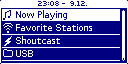
\includegraphics[width=128px]{images/home.png}}
\fcolorbox{white}{LCDBlue}{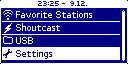
\includegraphics[width=128px]{images/home2.png}}

\begin{itemize}
 \item \textbf{Now Playing} Zeigt Informationen über das im Moment abgespielte Lied an. Hier kann auch der ``Snooze'' Modus gestartet werden. 
 \item \textbf{Favorite Stations} Liste der Lieblingsstationen. Von hier können Stationen abgespielt werden und es kann die Zuordnung zu den Favoriten Tasten 1-4 geändert werden. 
 \item \textbf{Shoutcast} Zugriff auf die SHOUTcast Services (Suchen von Stationen, Top Stationen, Zufalls Stationen und Genre Liste).
 \item \textbf{USB} Zugriff auf das angesteckte USB-Medium zum Abspielen von lokalen Liedern. 
 \item \textbf{Settings} Einstellungen für das Webradio, u.a. WLAN, Sprache, Lautstärke, Favoritenverwaltung.
\end{itemize}

\section{Now Playing}

Der ``Now Playing'' Bildschirm zeigt die Informationen zu dem aktuell abgespielten Lied bzw. Stream an. Wird momentan nichts abgespielt, wird folgender Bildschirm angezeigt

\fcolorbox{white}{LCDBlue}{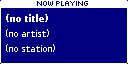
\includegraphics[width=128px]{images/now_playing_none.png}}

\subsection{Stream Wiedergabe}

Bei der Wiedergabe eines Streams steht der Titel des Liedes in der ersten Zeile, in der mittleren Zeile wird der Interpret angezeigt und die letzte Zeile enthält den Namen der Station.

\fcolorbox{white}{LCDBlue}{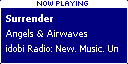
\includegraphics[width=128px]{images/now_playing.png}}

Ist einer der Zeilen zu lang um vollständig angezeigt zu werden, kann mit dem Drehrad eine Zeile ausgewählt werden. Dadurch wechselt diese in den Scroll-Modus und zeigt dadurch den gesamten Inhalt an.

\fcolorbox{white}{LCDBlue}{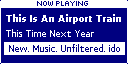
\includegraphics[width=128px]{images/now_playing_scroll.png}}


\subsubsection{Schlummermodus}
Befindet man sich im ``Now Playing'' Bildschirm, gelangt man durch Drücken des Drehrades (OK) in das Menü, in welchem man den Schlummermodus starten kann.

\fcolorbox{white}{LCDBlue}{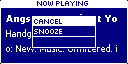
\includegraphics[width=128px]{images/now_playing_menu.png}}

Wählt man ``Snooze'' aus, öffnet sich ein neuer Bildschirm, auf dem man eingeben kann, wie viele Minuten die Musik weiter gespielt wird, bis sie sich selbst beendet. 
Die Minuten werden mit dem Drehrad ausgewählt, mit einem Druck auf das Drehrad (OK) wird bestätigt. Soll der Schlummermodus deaktiviert werden, stellt man 0 ein. 

\fcolorbox{white}{LCDBlue}{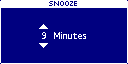
\includegraphics[width=128px]{images/snooze.png}}

Wenn der Schlummermodus aktiviert ist, kann man dies an dem Symbol (
\includegraphics[width=8px]{images/snooze_symbol.png}) rechts oben in der Statusleiste erkennen.

\fcolorbox{white}{LCDBlue}{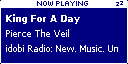
\includegraphics[width=128px]{images/snooze_activated.png}}


\subsubsection{Aktuellen Stream zu Favoriten}
Spielt man eine Station ab, die man nicht in den Favoriten gespeichert hat, zeigt das Menü, das man durch Drücken des Drehrades (OK) erhält eine zusätzliche Option an. 
Wählt man die Option ``As Favorite'' wird die aktuelle Station in die Favoritenliste aufgenommen. 

\fcolorbox{white}{LCDBlue}{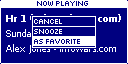
\includegraphics[width=128px]{images/now_playing_menu1.png}}

\subsection{USB Wiedergabe}

Erfolgt die Wiedergabe von einem USB-Medium, ändert sich der Aufbau des Bildschirms etwas. In der ersten und zweiten Zeile werden weiterhin Liedtitle und Interpret angezeigt, in der letzten Zeile 
steht allerdings immer ``USB''. Weiters gibt es einen ``Next'' Button. Durch Drücken des Drehrades (OK) wird zum nächsten Lied weitergeschaltet, falls ein Ordner oder eine Playlist abgespielt wird. 

\fcolorbox{white}{LCDBlue}{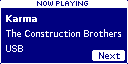
\includegraphics[width=128px]{images/usb_play.png}}

Ist kein ID3 Tag vorhanden, oder kann dieser aus irgend einem Grund nicht gelesen werden, werden für Titel und Interpret ``(no title)'' bzw. ``(no artist)'' angezeigt.

\fcolorbox{white}{LCDBlue}{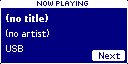
\includegraphics[width=128px]{images/usb_no_id3.png}}


Schlummermodus und Favoriten sind für USB Wiedergabe nicht verfügbar!



\section{Favorite Stations}
Hier werden jene Stationen angezeigt, die zu den Favoriten hinzugefügt wurden. Stationen werden mit dem Drehrad ausgewählt, ein Druck auf das Drehrad (OK) startet die Station. 
Die Stationsliste bleibt nach dem Starten jedoch geöffnet. Um wieder zurück auf den Hauptbildschirm zu kommen muss die Home-Taste gedrückt werden. 

\fcolorbox{white}{LCDBlue}{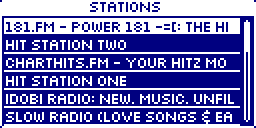
\includegraphics[width=128px]{images/stations.png}}

\subsection{Favoriten Zuordnung}
In diesem Menü erfolgt auch die Zuordnung von vier Stationen zu den Tasten 1-4. Um eine Station einer Taste zuzuordnen wählt man diese mit dem Drehrad aus, und drückt dann lange auf die 
gewünschte Taste (1-4), bis die Tastennummer rechts von der Station angezeigt wird:

\fcolorbox{white}{LCDBlue}{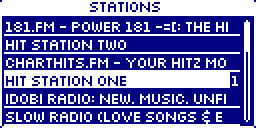
\includegraphics[width=128px]{images/stations_favorite.png}}

Jeder Taste kann genau eine Station zugeordnet werden. Um einer Taste eine neue Station zuzuweisen muss nur die neue Station ausgewählt werden und die Taste erneut lang gedrückt werden, damit die 
Zuordnung verändert wird. 

\subsection{Abspielen von Favoriten}
Stationen, die einer der Favoriten Tasten (1-4) zugeordnet wurden, können jederzeit mit einem Druck auf die entsprechende Taste gestartet werden. 



\section{Shoutcast}
Das Shoutcast Menü stellt die Funktionalitäten des SHOUTcast Services zur Verfügung. 

\fcolorbox{white}{LCDBlue}{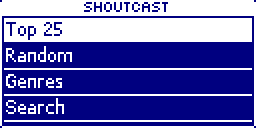
\includegraphics[width=128px]{images/shoutcast.png}}

\subsection{Top 25}
Hier werden die Top 25 SHOUTcast Stationen weltweit angezeigt. Durch Auswählen des Menüpunktes ``$<$ Back'' gelangt man wieder zurück in das Shoutcast Menü. Wählt man eine Station aus und drückt das Drehrad (OK) 
öffnet sich das Stations-Menü, auf das weiter unten eingegangen wird. 

\fcolorbox{white}{LCDBlue}{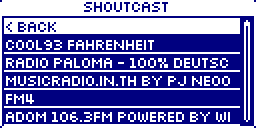
\includegraphics[width=128px]{images/shoutcast_top25.png}}


\subsection{Random}
In diesem Menü werden bei jedem Aufruf 30 zufällig ausgewählte Shoutcast Stationen angezeigt. Durch Auswählen des Menüpunktes ``$<$ Back'' gelangt man wieder zurück in das Shoutcast Menü. Wählt man eine Station aus und drückt das Drehrad (OK) 
öffnet sich das Stations-Menü, auf das weiter unten eingegangen wird. 

\subsection{Genres}
Ein Klick auf Genres zeigt eine Liste aller verfügbarer Hauptgenres an. 

\fcolorbox{white}{LCDBlue}{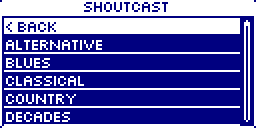
\includegraphics[width=128px]{images/shoutcast_genres.png}}

Die Auswahl des Genres führt dann - je nach Genre - zur Auswahl eines Untergenres oder zur Liste der Stationen, die diesem (Unter-)Genre zugeordnet sind.

\fcolorbox{white}{LCDBlue}{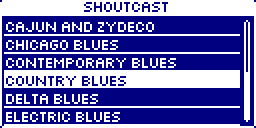
\includegraphics[width=128px]{images/shoutcast_subgenre.png}}


\subsection{Search}
In diesem Menü können SHOUTcast Stationen anhand von Stichworten gesucht werden. 

\fcolorbox{white}{LCDBlue}{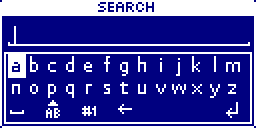
\includegraphics[width=128px]{images/shoutcast_search.png}}

Buchstaben werden mit dem Drehrad ausgewählt und mit einem Druck (OK) bestätigt. Die Symbole in der untersten Zeile haben folgende Funktionen.
\begin{itemize}
 \item 
\includegraphics[width=7px]{images/space.png} fügt ein Leerzeichen ein
 \item 
\includegraphics[width=7px]{images/upper.png} wechselt zu Großbuchstaben
 \item 
\includegraphics[width=7px]{images/numbers.png} wechselt zu Zahlen und Sonderzeichen
 \item 
\includegraphics[width=7px]{images/back.png} löscht das letzte Zeichen
 \item 
\includegraphics[width=7px]{images/enter.png} bestätigt die Eingabe und sucht nach entsprechenden Stationen
\end{itemize}


\subsection{Stations-Menü}
Wird eine SHOUTcast Station durch Druck auf das Drehrad (OK) ausgewählt, öffnet sich das Stations-Menü

\fcolorbox{white}{LCDBlue}{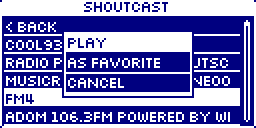
\includegraphics[width=128px]{images/shoutcast_menu.png}}

Hier kann zwischen den Optionen ``Play'' und ``As Favorite'' gewählt werden. ``Play'' spielt die Station ab, ``As Favorite'' fügt sie zur Favoriten-Liste hinzu, spielt sie jedoch nicht ab. 
Die Stationsliste bleibt nach der Auswahl einer Option weiterhin angezeigt. Wird eine Station abgespielt, kann sie auch im Nachhinein noch im ``Now Playing'' Bildschirm zu den Favoriten hinzugefügt werden. 


\section{USB}
Im USB Menü kann auf lokale Lieder zugegriffen werden, die sich auf einem angeschlossenem USB Medium befinden. Ist kein USB-Medium angeschlossen, das Medium wird nicht unterstützt oder es wurden keine Lieder gefunden 
wird eine leere Liste angezeigt:

\fcolorbox{white}{LCDBlue}{
\includegraphics[width=128px]{images/usb_empty.png}}

Der USB Modus unterstützt Unterordner und Playlists. Unterstützte Lieder werden mit einem Noten-Symbol markiert (
\includegraphics[width=5px]{images/song.png}), 
Playlists mit einem CD-Symbol (
\includegraphics[width=5px]{images/playlist.png}) und Ordner haben kein Symbol. Nicht unterstützt Dateiformate werden nicht angezeigt. 

\fcolorbox{white}{LCDBlue}{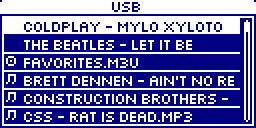
\includegraphics[width=128px]{images/usb_list.png}}

Von einem Unterordner kommt man durch Auswählen des ersten Menüpunktes (
\includegraphics[width=5px]{images/up.png} ..) wieder in den übergeordneten Ordner.

\fcolorbox{white}{LCDBlue}{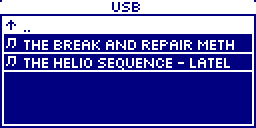
\includegraphics[width=128px]{images/usb_subfolder.png}}

\subsection{Abspielen von Liedern und Playlists}
Um ein einzelnes Lied oder eine Playlist abzuspielen markiert man den Eintrag in der Liste und bestätigt mit einem Druck auf das Drehrad (OK). Die aktuelle Liste bleibt geöffnet und das Lied wird abgespielt.

\subsection{Abspielen von Ordnern}
Durch Drücken der Play/Stop-Taste wird eine Playlist aus allen Liedern im aktuellen Ordner in zufälliger Reihenfolge erstellt und abgespielt. 


\section{Settings}

Im Settings Menü können diverse Einstellungen vorgenommen werden.

\fcolorbox{white}{LCDBlue}{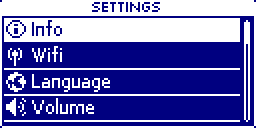
\includegraphics[width=128px]{images/settings1.png}}
\fcolorbox{white}{LCDBlue}{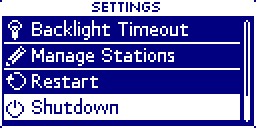
\includegraphics[width=128px]{images/settings2.png}}

\subsection{Info}
Hier werden Informationen zum aktuellen Status des Geräts angezeigt. Durch einen Druck auf das Drehrad (OK) kommt man wieder zum Settings-Menü.

\fcolorbox{white}{LCDBlue}{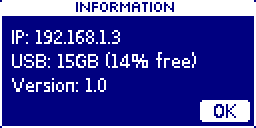
\includegraphics[width=128px]{images/settings_info.png}}

\begin{itemize}
 \item Die IP-Adresse des Geräts, oder ``not available'' wenn keine IP-Adresse gefunden wurde oder das Gerät nicht mit dem Internet verbunden ist.
 \item Die Kapazität (in GB) des angesteckten USB-Mediums und wie viel freier Speicher noch vorhanden ist (in Prozent).
 \item Die Version der Software.
\end{itemize}


\subsection{WiFi}
Falls die Internetverbindung über einen WLAN Stick hergestellt werden soll, kann hier die Verbindung eingerichtet werden. Die Auwahl startet das Suchen nach verfügbaren Access Points.

\fcolorbox{white}{LCDBlue}{
\includegraphics[width=128px]{images/settings_wifi_scanning.png}}
\fcolorbox{white}{LCDBlue}{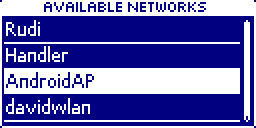
\includegraphics[width=128px]{images/settings_wifi.png}}

Es werden nur Access Points mit WPA-Verschlüsselung unterstützt.
Wird ein Access Point ausgewählt, folgt eine Aufforderung zur Eingabe des Passworts

\fcolorbox{white}{LCDBlue}{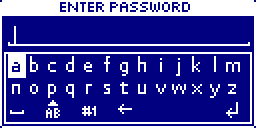
\includegraphics[width=128px]{images/settings_wifi_password.png}}

Nach dem Verbindsversuch wird der Info-Bildschrim angezeigt, auf dem man die IP-Adresse sehen kann bzw. ein ``not available'' wenn die Verbindung fehlschlug. 


\subsection{Language}
In diesem Menü kann die Sprache des Geräts geändert werden. Wird die ausgewählte Sprache durch Drücken des Drehrades (OK) bestätigt, ist diese sofort aktiv und das Settings Menü wird wieder angezeigt.

\fcolorbox{white}{LCDBlue}{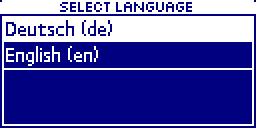
\includegraphics[width=128px]{images/settings_language.png}}

\subsection{Volume}
Hier kann die Lautstärke des Audio Ausgangs verändert werden. Es wird empfohlen die Lautstärke auf ca. 70\% zu setzen und die Musiklautstärke direkt an der angeschlossenen Stereoanlage oder den Lautsprechern zu ändern. 

\fcolorbox{white}{LCDBlue}{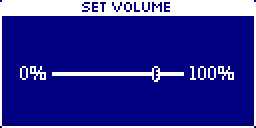
\includegraphics[width=128px]{images/settings_volume.png}}

Die Lautstärke wird durch Drehen des Drehrades verändert und sofort übernommen. Durch Drücken des Drehrades gelangt man zurück in das Settings-Menü. 

\subsection{Backlight Timeout}
Die Zeitdauer, welche die Hintergrundbeleuchtung des Displays eingeschaltet ist kann hier verändert werden. Die Zeit ist in Sekunden angegeben und wird gemessen seit der letzten Benutzerinteraktion 
(drücken einer Taste, drehen des Drehrades). Im Now-Playing-Bildschirm wird die Hintergrundbeleuchtung nie ausgeschaltet. 

\fcolorbox{white}{LCDBlue}{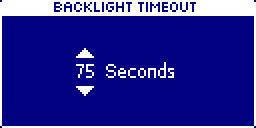
\includegraphics[width=128px]{images/settings_backlight.png}}

Das Timeout wird durch Drehen des Drehrades verändert und durch Drücken des Drehrades (OK) gespeichert. Nach dem Speichern wird das Settings-Menü angezeigt. 


\subsection{Manage Stations}
Dieser Menüpunkt erlaubt das Ändern der Favoriten Liste. Beim Öffnen werden alle Favoriten angezeigt. 

\fcolorbox{white}{LCDBlue}{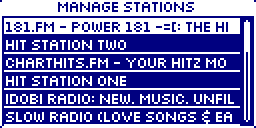
\includegraphics[width=128px]{images/settings_manage.png}}

Stationen können mit Hilfe des Drehrades ausgewählt werden. Durch Drücken des Drehrades (OK) öffnet sich ein Menü. 

\fcolorbox{white}{LCDBlue}{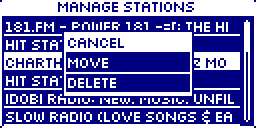
\includegraphics[width=128px]{images/settings_manage_menu.png}}

\subsubsection{Löschen von Stationen}
Wählt man die Option ``Delete'' im Menü aus, wird die Station aus der Favoriten Liste gelöscht. 
Diese Aktion kann nicht rückgängig gemacht werden!

\subsubsection{Verschieben von Stationen}
Wählt man die Option ``Move'' kann die Reihenfolge der Station verändert werden. Dabei erscheint eine Markierung (
\includegraphics[width=6px]{images/marker.png}) neben dem Stationsnamen. 

\fcolorbox{white}{LCDBlue}{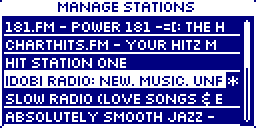
\includegraphics[width=128px]{images/settings_manage_move_start.png}}

Die Position der Station kann verändert werden, indem am Drehrad gedreht wird. Ist die Station an der gewünschten Position, 
wird sie durch einen Druck auf das Drehrad (OK) hier fixiert und die Markierung verschwindet wieder. 

\subsection{Restart}
Ein Klick auf Restart startet die Firmware neu und beendet alle laufenden Streams. Falls sich die Musik nicht mehr beenden lasst sollte dieser schnelle Neustart helfen. 

\subsection{Shutdown}
Soll das Gerät vom Strom getrennt werden, sollte man es vorher herunterfahren um Datenverlust zu vermeiden. Dies geht mit diesem Menüpunkt. 
Das Herunterfahren dauert ungefähr eine Minute, danach kann das Internet Radio gefahrlos vom Strom getrennt werden. 


\chapter{Fernsteuerung}

\section{Android}
Das Gerät verfügt auch über die Möglichkeit der Fernsteuerung durch eine Applikation für Android. Diese App kann von der Projektseite heruntergeladen und auf 
jedem Android Gerät mit einer Android Version ab 2.1 installiert werden. 

Wird die Android App gestartet, wird automatisch das Webradio über Zeroconf gesucht und wenn es gefunden wurde, wird der Hauptbildschirm angezeigt.

\fcolorbox{white}{white}{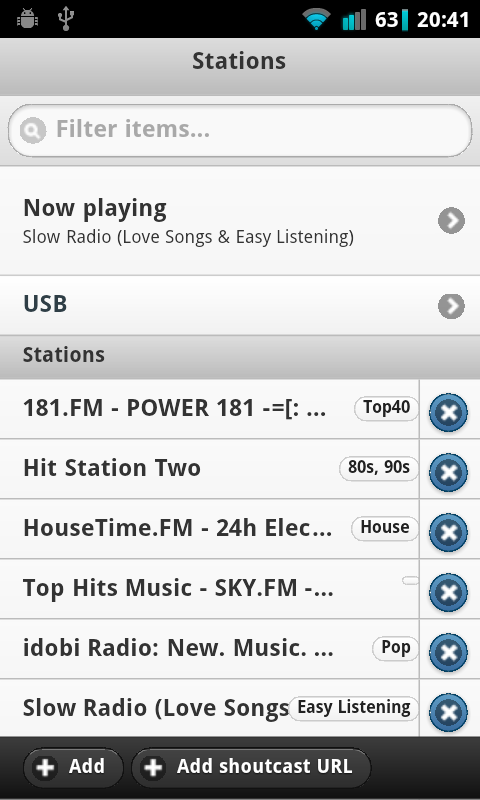
\includegraphics[width=120px]{images/android_home.png}}

Hier sieht man die Liste der Favoriten, kann diese über das Feld ``Filter items...'' durchsuchen, auf ein angestecktes USB-Medium zugreifen und die Informationen zu dem aktuellen Lied anzeigen. 
Weiters ist es möglich, eigene nicht-SHOUTcast Stationen hinzuzufügen sowie SHOUTcast Stationen hinzuzufügen. 

\subsection{Now Playing}
Hier wird das aktuell abgespielte Lied angezeigt. Neben dem Liedtitel, dem Interpreten und der Radio Station wird auch noch - falls verfügbar - ein Foto des Interpreten angezeigt. 

\fcolorbox{white}{white}{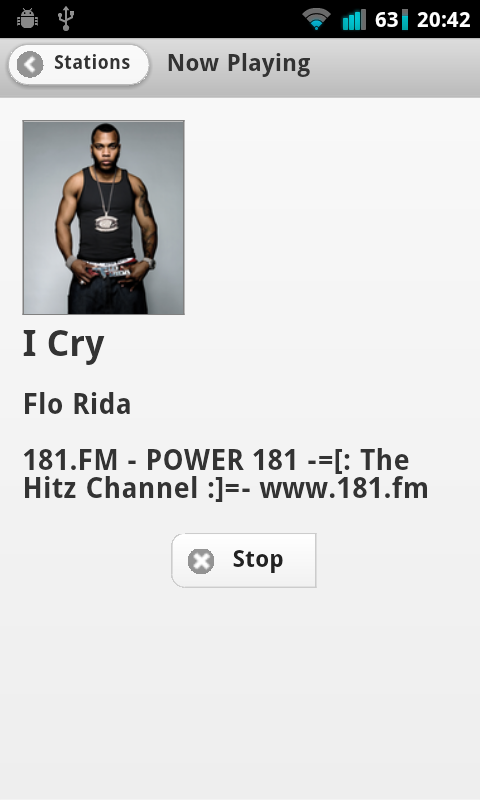
\includegraphics[width=120px]{images/android_now_playing.png}}

Ein Klick auf den ``Stop''-Button beendet die aktuelle Wiedergabe. 
Mit dem Button ``Stations'' gelangt man zurück auf die Hauptseite. 

\subsection{USB}
\fcolorbox{white}{white}{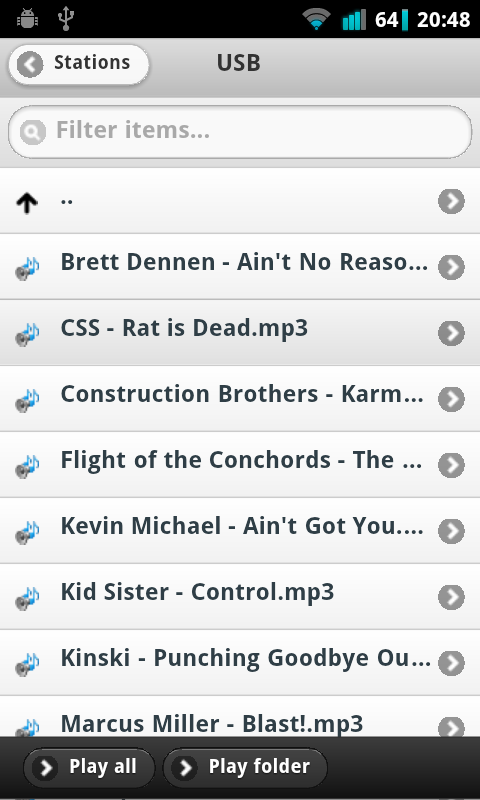
\includegraphics[width=120px]{images/android_usb.png}}

Dieser Menüpunkt erlaubt den Zugriff auf ein angeschlossenes USB-Medium. Lieder können direkt mit einem Klick abgespielt werden. 
Unterordner werden unterstützt und mit einem Ordner Symbol (
\includegraphics[width=12px]{images/folder.png}) gekennzeichnet. Mit einem Klick auf den ersten Eintrag 
(
\includegraphics[width=7px]{images/arrow_up.png}..) gelangt man in den übergeordneten Ordner. Mit dem Button ``Stations'' gelangt man zurück auf die Hauptseite. 

\subsubsection{Abspielen von Ordner}
Um alle Lieder im aktuellen Ordner wiederzugeben klickt man auf ``Play folder''. 

\subsection{Stationen}
Auf der Startseite gibt eine Liste der Lieblingsstationen. Diese können mit einem Klick gestartet werden. 

\subsubsection{Station hinzufügen}
Es ist auch möglich, neue Stationen hinzuzufügen. Mit ``Add'' wird eine nicht-SHOUTcast Station hinzugefügt. 

\fcolorbox{white}{white}{\includegraphics[width=120px]{images/android_add_station.png}}
\fcolorbox{white}{white}{\includegraphics[width=120px]{images/android_add_shoutcast.png}}

Dabei müssen ein Name (der in der Favoriten Liste angezeigt wird), Genre (wird nur in der Android App und auf der mobilen Website angezeigt) und die URL der Station angegeben werden. 
Die Station wird dann zu den Favoriten hinzugefügt. 

Es können auch SHOUTcast Stationen hinzugefügt werden. Hier muss nur die URL angegeben werden, Name und Genre sind optional. Die URL hat die Form \url{http://yp.shoutcast.com/sbin/tunein-station.pls?id=65456}. 
Man erhält sie, wenn man auf der Seite \url{http://www.shoutcast.com/} den Link zu einer Station kopiert. 

\subsubsection{Station löschen}
Eine Station kann gelöscht werden indem man das Löschen-Symbol (\includegraphics[width=12px]{images/delete.png}) anklickt. 

\section{Website}

\includegraphics[width=0.80\linewidth]{images/website.png}

Die Webseite bietet im Grunde die gleiche Funktionalität wie die Android App und kann sowohl von einem PC als auch von einem mobilen Browser aufgerufen werden. 
Als URL kann entweder die IP-Adresse des Gerätes verwendet werden (bei Settings - Info zu finden) oder die Zeroconf URL \url{http://raspberrypi.local}.

\end{document}
